Lots of beverage consumers lose track of their collection sof drinks and this can lead to a major loss of money and shelf space. We 
decided to use a dataset which contains the data for a variety of rare beer to design our drinks database. The user will 
be able to scan the beer the purchased using an in-built barcode scanner in the app and assign the drink to an empty 
portion of the shelf.  

    Our system will need access to the phones camera, which will only be active when the user wants to scan the bar code.
The system will search for the information of the drink using the barcode in the dataset and populate the shelves on the application with the required data.

    The expiration date of the beer and the number of that type of beer in the shelves will be kept track of so as to handle the user requests, and also 
send push notifications to the user when the beer is low on supply or about to expire.

    Furthermore, the user can modify the functionality of the app (i.e the notifications sound, details of each shelf) within the app.

\begin{figure}[ht]
    \centering
    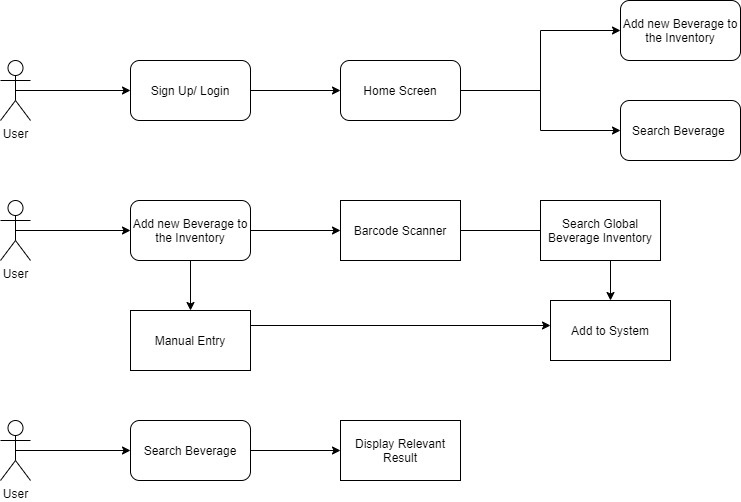
\includegraphics[width=0.5\textwidth]{images/systemoverview}
    \caption{High Level system overview of major system components}
\end{figure}